\chapter{METODOLOGI}

% Ubah konten-konten berikut sesuai dengan isi dari metodologi

\section{Metode yang digunakan}

% Contoh input gambar dengan format *.jpg
\begin{figure} [ht] \centering
  % Nama dari file gambar yang diinputkan
  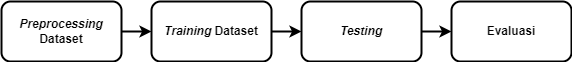
\includegraphics[scale=0.75]{gambar/metodologi.png}
  % Keterangan gambar yang diinputkan
  \caption{Diagram Desain Sistem}
  % Label referensi dari gambar yang diinputkan
  \label{fig:DiagramMetodologi}
\end{figure}

\subsection{\emph{Preprocessing} Dataset}

Pada tahap ini, dataset yang sudah ada akan melalui beberapa proses terlebih dahulu sebelum memasuki tahap \emph{training}. Beberapa proses tersebut diantaranya adalah membersihkan dataset, augmentasi gambar, dan pembagian dataset. Hal tersebut dilakukan agar proses \emph{training} menjadi lebih optimal.

\subsection{\emph{Training} Dataset}

Dataset yang sudah diproses pada tahap \emph{preprocessing} akan dilakukan \emph{training} menggunakan metode CNN. Hasil dari tahap ini berupa model CNN yang dapat melakukan reidentifikasi kendaraan.

\subsection{\emph{Testing}}

Testing dilakukan untuk menguji model yang sudah dibuat. Apabila hasil kurang sesuai, maka akan dilakukan training lagi untuk mendapatkan model yang lebih baik dan hasil testing bisa lebih akurat. Testing akan menggunakan citra baru atau citra yang belum digunakan dalam tahap training. Hal ini untuk benar-benar menguji keberhasilan model yang sudah dibuat.

\subsection{Evaluasi}

Pada tahap ini, seluruh proses penelitian yang sudah dilakukan akan dievaluasi. Proses evaluasi juga meliputi penarikan kesimpulan dan menentukan kelayakan model dalam melakukan reidentisikasi kendaraan.

\section{Data dan peralatan yang digunakan}

\begin{enumerate}[label=(\alph*)]
  \item Dataset
        \begin{figure} [ht] \centering
          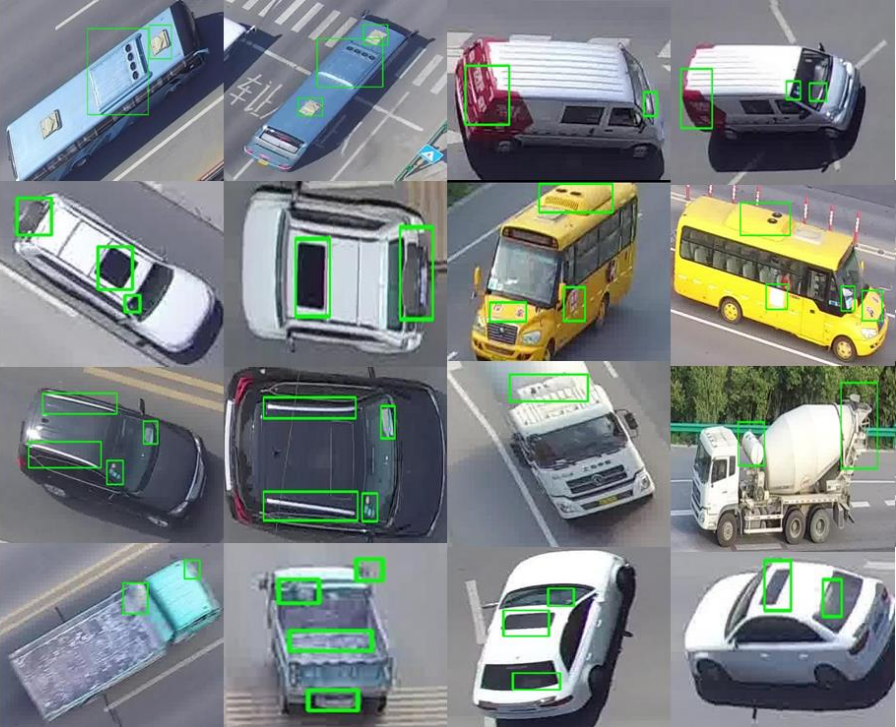
\includegraphics[scale=0.4]{gambar/VRAI-dataset.png}
          \caption{Sampel Citra yang Ada pada Dataset VRAI}
          \label{fig:VRAIDatset}
        \end{figure}

        Dataset yang digunakan pada penelitian ini merupakan dataset yang diambil dari repositori publik github milik JiaoBL1234 \cite*{VRAIDatasetGithub}. Berdasarkan paper yang berjudul ”Vehicle Re-identification in Aerial Imagery: Dataset and Approach”, Peng Wang et al membuat dataset untuk reidentifikasi kendaraan dengan mengaplikasikan UAV sebagai alat pengambil citra. Dataset tersebut diberi nama Vehicle Re-identification for Aerial Image (VRAI). Dataset VRAI terdiri dari 137.613 gambar dari 13.022 sampel kendaraan. Gambar dari setiap sampel kendaraan ditangkap oleh kamera dari dua UAV bermerek DJI di lokasi yang berbeda, dengan berbagai sudut pandang dan ketinggian terbang (15m hingga 80m) \cite{Wang2019vehicle}.

        \newpage

  \item Laptop

        Laptop digunakan untuk pengerjaan penelitian ini, mulai dari \emph{Preprocessing} Dataset, \emph{Training} Dataset, \emph{Testing}, maupun penyusunan laporan. Laptop yang digunakan adalah laptop pribadi milik penulis. Adapun merek dari laptop yang digunakan adalah Lenovo Legion 5 tipe 15ARH05H dengan spesifikasi sebagai berikut:
        \begin{longtable}{|c|c|c|}
          \caption{Spesifikasi Laptop}
          \label{tb:spesifikasilaptop}                    \\
          \hline
          % \rowcolor[HTML]{C0C0C0}
          \textbf{Tipe}      & \textbf{Detail}            \\
          \hline
          \textit{Processor} & AMD Ryzen 7 4800H          \\
          Memory             & 16 GB                      \\
          Storage            & SSD 1TB                    \\
          Graphic Card       & NVIDIA GeForce GTX 1660 Ti \\
          Operating System   & Windows 11                 \\
          \hline
        \end{longtable}
  \item Google Colaboratory

        Google Colaboratory atau biasa disebut "Google Colab" adalah produk dari Google Research. Google Colab memungkinkan siapa saja untuk menulis dan mengeksekusi kode python arbitrer melalui browser, dan sangat cocok untuk pembelajaran mesin, analisis data, dan pendidikan \cite{GoogleColab}. Pada penelitian ini, Google Colab digunakan sebagai \emph{platform} untuk menulis semua kode program dan juga untuk melakukan penelitian khususnya dalam preprocessing data, training data, dan testing data.
\end{enumerate}

\newpage

\section{Urutan pelaksanaan penelitian}

Penelitian ini akan dilaksanakan selama 16 minggu. Urutan pelaksanaan penelitian ini dapat dilihat pada tabel \ref{tb:TimelinePenelitian}.
% Ubah tabel berikut sesuai dengan isi dari rencana kerja
\newcommand{\w}{}
\newcommand{\G}{\cellcolor{gray}}
\begin{table}[h!]
  \caption{\label{tb:TimelinePenelitian}\emph{Timeline} Penelitian}
  \begin{tabular}{|p{3.5cm}|c|c|c|c|c|c|c|c|c|c|c|c|c|c|c|c|}

    \hline
    \multirow{2}{*}{Kegiatan} & \multicolumn{16}{|c|}{Minggu}                                                                       \\
    \cline{2-17}              &
    1                         & 2                             & 3  & 4  & 5  & 6  & 7  & 8  & 9  & 10 & 11 & 12 & 13 & 14 & 15 & 16 \\
    \hline

    % Gunakan \G untuk mengisi sel dan \w untuk mengosongkan sel
    Studi Literatur           &
    \G                        & \G                            & \w & \w & \w & \w & \w & \w & \w & \w & \w & \w & \w & \w & \w & \w \\
    \hline

    Preprocessing Data        &
    \w                        & \w                            & \G & \G & \G & \w & \w & \w & \w & \w & \w & \w & \w & \w & \w & \w \\
    \hline

    Training data             &
    \w                        & \w                            & \w & \w & \G & \G & \G & \G & \G & \G & \G & \G & \G & \w & \w & \w \\
    \hline

    Testing                   &
    \w                        & \w                            & \w & \w & \w & \w & \w & \w & \w & \w & \G & \G & \G & \w & \w & \w \\
    \hline

    Evaluasi                  &
    \w                        & \w                            & \w & \w & \w & \w & \w & \w & \w & \w & \w & \w & \w & \G & \G & \w \\
    \hline

    Pembuatan Laporan         &
    \G                        & \G                            & \G & \G & \G & \G & \G & \G & \G & \G & \G & \G & \G & \G & \G & \G \\
    \hline
  \end{tabular}
\end{table}
